The Proposed solution will consist of four parts:

\begin{enumerate}
    \item A dataset consisting of public Instagram images which will
    be discussed in section \ref{Dataset}
    \item A trained Convolutional Neural Network (CNN) model to
    predict the image category. A prototype of this model will be
    discussed in section \ref{Evaluation}.
    \item A method for calculating the scores of activities
    \item A genetic algorithm which is able to produce itineraries in
    reasonable time and with a high score.
\end{enumerate}


\begin{figure}[H]
    % \caption{The image shows a sample image form each of the category}
    \centering
    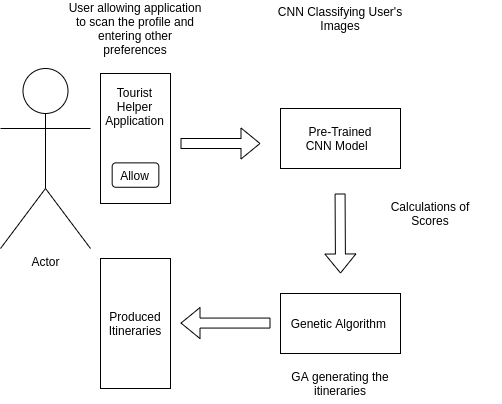
\includegraphics[scale=0.45]{Diagram.png}
    \label{diagram}
\end{figure}